%NEURAL PRESY ;)

%----------------------------------------------------------------------------------------
%   PACKAGES AND THEMES
%----------------------------------------------------------------------------------------

\documentclass[table]{beamer}

\usefonttheme{professionalfonts}
\usefonttheme[onlymath]{serif}

\mode<presentation> {

\usetheme{Berkeley}
%\setbeamertemplate{footline} % To remove the footer line in all slides uncomment this line
%\setbeamertemplate{footline}[page number] % To replace the footer line in all slides with a simple slide count uncomment this line

\setbeamertemplate{navigation symbols}{} % To remove the navigation symbols from the bottom of all slides uncomment this line
}

\usepackage{graphicx} % Allows including images
\usepackage{booktabs} % Allows the use of \toprule, \midrule and \bottomrule in tables
\usepackage{caption}
\usepackage{subcaption}
\usepackage{algorithm,algorithmic}

% tikz and associated macros
\usepackage{tikz}
\usepackage{tikz-cd}

\usepackage{pgfplots}
\def\layersep{2cm}
\def\nodesep{0.25cm}
\newcommand*{\Scale}[2][4]{\scalebox{#1}{$#2$}}%
\newcommand*{\Resize}[2]{\resizebox{#1}{!}{$#2$}}%
\newcommand\sep{1.9cm}
\newcommand\height{0.9cm}
\usetikzlibrary{decorations.pathmorphing, backgrounds}
\tikzset{snake it/.style={decorate, decoration=snake}}

%
%

% math
\usepackage{amsthm}

 \usepackage{relsize}
\usepackage{amsmath}
\usepackage{amssymb}
\usepackage{mathabx}
\usepackage{xcolor}

\numberwithin{equation}{subsection}
\numberwithin{theorem}{subsection}

\DeclareSymbolFont{cmlargesymbols}{OMX}{cmex}{m}{n}
\let\sumop\relax
\DeclareMathSymbol{\sumop}{\mathop}{cmlargesymbols}{"50}


\def\reals{{\mathbb R}}
\def\torus{{\mathbb T}}
\def\integers{{\mathbb Z}}
\def\rationals{{\mathbb Q}}
\def\expect{\mathop{{\mathbb{E}}}}
\def\tens{\mathop{{\bigotimes}}}
\def\naturals{{\mathbb N}}
\def\complex{{\mathbb C}\/}
\def\distance{\operatorname{distance}\,}
\def\support{\operatorname{support}\,}
\def\dist{\operatorname{dist}\,}
\def\Span{\operatorname{span}\,}
\def\degree{\operatorname{degree}\,}
\def\kernel{\operatorname{kernel}\,}
\def\dim{\operatorname{dim}\,}
\def\codim{\operatorname{codim}}
\def\trace{\operatorname{trace\,}}
\def\dimension{\operatorname{dimension}\,}
\def\codimension{\operatorname{codimension}\,}
\def\kernel{\operatorname{Ker}}
\def\Re{\operatorname{Re\,} }
\def\Im{\operatorname{Im\,} }
\def\eps{\varepsilon}
\def\lt{L^2}
\def\bull{$\bullet$\ }
\def\det{\operatorname{det}}
\def\Det{\operatorname{Det}}
\def\diameter{\operatorname{diameter}}
\def\symdif{\,\Delta\,}
\newcommand{\norm}[1]{ \|  #1 \|}
\newcommand{\set}[1]{ \left\{ #1 \right\} }
\def\suchthat{\mathrel{}\middle|\mathrel{}}
\def\one{{\mathbf 1}}
\def\cl{\text{cl}}

\def\newbull{\medskip\noindent $\bullet$\ }
\def\nobull{\noindent$\bullet$\ }
\def\defeq{\stackrel{\text{def}}{=}}


\newcommand{\argmin}{\mathop{\mathrm{argmin}}} 
\newcommand{\argmax}{\mathop{\mathrm{argmax}}} 


\def\scriptf{{\mathcal F}}
\def\scriptq{{\mathcal Q}}
\def\scriptg{{\mathcal G}}
\def\scriptm{{\mathcal M}}
\def\scriptb{{\mathcal B}}
\def\scriptc{{\mathcal C}}
\def\scriptt{{\mathcal T}}
\def\scripti{{\mathcal I}}
\def\scripte{{\mathcal E}}
\def\scriptv{{\mathcal V}}
\def\scriptw{{\mathcal W}}
\def\scriptu{{\mathcal U}}
\def\scriptS{{\mathcal S}}
\def\scripta{{\mathcal A}}
\def\scriptr{{\mathcal R}}
\def\scripto{{\mathcal O}}
\def\scripth{{\mathcal H}}
\def\scriptd{{\mathcal D}}
\def\scriptl{{\mathcal L}}
\def\scriptn{{\mathcal N}}
\def\scriptp{{\mathcal P}}
\def\scriptk{{\mathcal K}}
\def\scriptP{{\mathcal P}}
\def\scriptj{{\mathcal J}}
\def\scriptz{{\mathcal Z}}
\def\scripts{{\mathcal S}}
\def\scriptx{{\mathcal X}}
\def\scripty{{\mathcal Y}}
\def\frakv{{\mathfrak V}}
\def\frakG{{\mathfrak G}}
\def\frakB{{\mathfrak B}}
\def\frakC{{\mathfrak C}}
\def\ugearrow{{
  \mathlarger{
    \mathlarger{
      \mathlarger{
        \mathlarger{
          \mathlarger{
            \mathlarger{
              \mathlarger{
              \mathlarger{\implies}
              }
            }
          }
        }
      }
    }
  }
}}



%----------------------------------------------------------------------------------------
%   TITLE PAGE
%----------------------------------------------------------------------------------------

\title[Reinforcement Learning]{Bootcamp 6: Reinforcement Learning}

\author[Guss \& Bartlett]{\includegraphics[height=2cm,width=2cm]{BlueGold_fill_small.png}\\   William H. Guss, James Bartlett\\\{wguss, james\}@ml.berkeley.edu\\Machine Learning at Berkeley}
\date{April 22, 2016} % Date, can be changed to a custom date
\makeatletter
\newcommand{\verbatimfont}[1]{\renewcommand{\verbatim@font}{\ttfamily#1}}
\makeatother

\usefonttheme{professionalfonts}

\begin{document}
  

\begin{frame}{}
\titlepage
\end{frame}


\addtobeamertemplate{frametitle}{}{%
\begin{tikzpicture}[remember picture,overlay]
\node[anchor=north east,yshift=10pt] at (current page.north east) {\includegraphics[height=2cm]{White_outline_small_name_transparent.png}};
\end{tikzpicture}}

\begin{frame}

\frametitle{Overview}
\tableofcontents
\end{frame}


%----------------------------------------------------------------------------------------
%   PRESENTATION SLIDES
%----------------------------------------------------------------------------------------
\section{Introduction}
%!TEX root = ../pres.tex

\begin{frame}
  \frametitle{Problem: ML for Pacman.}
  \begin{columns}
    \begin{column}{0.5\textwidth}

    \onslide<1->{
    \emph{How would you solve pacman with machine learning?} } \\[0.9cm]

    \onslide<2->{
   \textbf{ Find a model which takes screen pixels to actions:}
    \begin{equation*}
      \pi_\theta: s_t \mapsto a_t.
    \end{equation*}}

    \onslide<3->{
      \emph{What is your loss function? Data?}
    }
   
    \end{column}
    \begin{column}{0.5\textwidth}
    \includegraphics[width=0.9\textwidth]{Pac-man.png}
    \end{column}
  \end{columns}
\end{frame}


\begin{frame}
  \frametitle{Problem: ML for Pacman.}
  \begin{columns}
    \begin{column}{0.5\textwidth}
    \begin{equation*}
    \ugearrow
    \end{equation*}
    \end{column}
    \begin{column}{0.5\textwidth}
    \includegraphics[width=0.9\textwidth]{Pac-man.png}
    \end{column}
  \end{columns}
\end{frame}




\begin{frame}
  \frametitle{Solution: Reinforcement Learning}
  \begin{columns}
    \begin{column}{0.5\textwidth}
      \begin{itemize}
        \item<1-> Supervised learning is \emph{not} the most general formulation of learning.
        \item<2-> Humans learn through reward and penalty
      \end{itemize}
    \end{column}
    \begin{column}{0.5\textwidth}
    \includegraphics[width=0.9\textwidth]{Pac-man.png}
    \end{column}
  \end{columns}
\end{frame}


\begin{frame}
  \frametitle{Solution: Reinforcement Learning}
  \begin{columns}
    \begin{column}{0.5\textwidth}
      \begin{itemize}
        \item<1-> Can we make algorithms which improve with crude reward signals?
      \end{itemize}
       \begin{center}
        \textbf{Machine learning without explicit objective functions}
        \begin{equation*}
        	\Downarrow
        \end{equation*}
        \textbf{Reinforcement Learning (RL)}
        \end{center}
    \end{column}
    \begin{column}{0.5\textwidth}
    \includegraphics[width=0.9\textwidth]{Pac-man.png}
    \end{column}
  \end{columns}
\end{frame}


\section{Theory}
%!TEX root = ../pres.tex
\begin{frame}
\frametitle{The Core Idea}
\begin{center}
  \includegraphics[width=0.5\textwidth]{reinforcementlearning.png}
\end{center}
\begin{itemize}
  \item Models (agents) take action $a_t$ in some environment.
  \item Environment provides state $s_t$, reward $r_t$.
  \item Models learn to maximize reward $r_t$, $\forall t$.
\end{itemize}
\end{frame}




\begin{frame}
  \frametitle{Markov Decision Process (MDP)}
      Environment, $E = (\mathcal{S}, \mathcal{A}, \mathcal{R}, \rho, r)$. 
        \begin{enumerate}
        \item State space, $\mathcal{S}$
        \item Action space, $\mathcal{A}$
        \item Reward space, $\mathcal{R}$   
        \item Transition distribution, $\rho(s'\ |\ s,a)$. Given a previous state $s$ and action $a$, environment gives $s'$.
        \item Reward function $r(s,a) \in \mathcal{R}$.
        \end{enumerate}
        \textbf{Markov Property:} $\rho(s'\ |\ s,a)$ depends only on $s,a$ not previous states!
\end{frame} 

\begin{frame}
  \frametitle{Markov Decision Process (MDP)}
  \begin{center}
  \textbf{Example MDP}
        \includegraphics[width=0.9\textwidth]{Markov_Decision_Process_example.png}
  \end{center}
\end{frame}



\begin{frame}
  \frametitle{Pacman as an MDP}
    \begin{columns}
    \begin{column}{0.5\textwidth}
      \begin{itemize}
        \item $\scripts = \mathbb{R}^{256\times 256},$ images as state space.
        \item $\scripta = \{\uparrow, \downarrow, \rightarrow, \leftarrow\}$, joystick as action space.
        \item $r(s_t,a_t) = $ change in score.
        \item $\rho(s_{t+1}\ |\ s_t, a_t) = $ next frame of game after joystick action $a_t$.
      \end{itemize}
    \end{column}
    \begin{column}{0.5\textwidth}
    \includegraphics[width=0.9\textwidth]{Pac-man.png}
    \end{column}
  \end{columns}
\end{frame}



\begin{frame}[fragile]
  \frametitle{Policies/Agents}
\textbf{Two different types of agents}
    \begin{itemize}
    \item Deterministic policy $a = \pi(s)$ acts in $E$. 
    \item Stochastic policy $a \sim \pi(a | s)$ gives a probability distibution over actions.
    \end{itemize}

\textbf{Policy Trajectories}
    
    \begin{equation*}
      \begin{tikzcd}
          s_1 \arrow{r}{\pi} & a_1 \arrow{r}{\rho, r} & s_2, r_2 \arrow{r}{\pi}& a_2  \arrow{r}{\rho, r} & \cdots
         \end{tikzcd}   
    \end{equation*}
\end{frame}



\begin{frame}
\frametitle{Value under a policy}
  The \textbf{state value} is a function of a given state for an agent $\pi$ defined as 
  \begin{equation*}
    V^\pi(s_t) = \mathbb{E}\left[\sum_{n={t+1}}^\infty \gamma^n r(s_n, \pi(s_n))\right]
  \end{equation*} 
  \begin{enumerate}
    \item $\gamma$ is the discount factor
    \item $\pi(s_n)$ is the action the agent $\pi$ makes after seeing state $s_n$.
    \item $r(s_n, \pi(s_n))$ is the reward the agent gets from taking that action.
  \end{enumerate}
\end{frame}

\begin{frame}
\frametitle{Value under a policy}
  The \textbf{state-action value} for an agent $\pi$ is defined such that
  \begin{equation*}
    Q^\pi(s_t, a_t) = \mathbb{E}\left[\underbrace{r(s_t, a_t)}_{\text{reward for } a_t} + V^\pi(s_t)\right]
  \end{equation*}
  \begin{itemize}
    \item Given some state $s_t$, the \emph{best} agent, $\pi^*$ is one that take action 
  \begin{equation*}
    a_t = \argmax_a Q(s_t, a).   
  \end{equation*}
  \end{itemize}
\end{frame}

\begin{frame}
  \frametitle{Problems in Reinforcement Learning}
  \begin{itemize}
    \item \textbf{Policy Optimization:} maximize the expected reward with respect to a policy $\pi$;
    \begin{equation*}
      \pi^* = \argmax_\pi \mathbb{E}\left[\sum_{t=0}^\infty r_t \right]
    \end{equation*}
    \item \textbf{Policy Evaluation:} Given some fixed policy $\pi$ compute expected return.
    \begin{itemize}
      \item Computing $Q^{\pi}$, $V^{\pi}$, and other expectations on policy rollout.
      \item Lets us perform policy optimization!
    \end{itemize}
  \end{itemize}
\end{frame}



\section{Algorithms}
\begin{frame}
\frametitle{$\ $}
  \begin{center}
    \Huge{\textbf{Assorted Algorithms}
    }
  \end{center}
  We'll go over:
  \begin{itemize}
    \item Behavioral Cloning
    \item Q-Learning
    \item Policy Iteration
  \end{itemize}
  
  Learn at home:
  \begin{itemize}
    \item Value iteration
    \item Temporal Difference Methods
    \item Inverse Reinforcement Learning.
  \end{itemize}

\end{frame}


%!TEX root = ../pres.tex

\begin{frame}
	\frametitle{Behavioral Cloning}
	\begin{center}
		\textbf{Behavioral Cloning:} Supervised learning in MDPs using and expert agent expert $\pi^*$!
	\end{center}
	Given expert examples $\scriptd = (s_t, a_t = \pi^*(s_t))$ and a model $\pi_\theta$ find $\theta^*$ st
	\begin{equation*}
		\theta^*  = \argmin_\theta \scriptl(a_t, \pi_\theta(s_t)).
	\end{equation*}
	where $\scriptl$ is some loss function.
	\begin{itemize}
		\item  Show, don't tell! 
		\item No complicated machinery, just standard ML.
	\end{itemize}
\end{frame}


\begin{frame}
	\frametitle{Behavioral Cloning}
		\textbf{Issue: Compounding Error}
		\begin{columns}
			\begin{column}{0.5\textwidth}
			Given some irreducible error $\epsilon =0.001$
				\begin{itemize}
					\item $\scriptl(a_0, \pi(s_0)) = \epsilon$
					\item $\scriptl(a_1, \pi(s_1)) = 2\epsilon$
					\item $\scriptl(a_2, \pi(s_2)) = 3\epsilon$
					\item $\scriptl(a_3, \pi(s_3)) = 4\epsilon$
					\item $\scriptl(a_4, \pi(s_4)) = 5\epsilon$
				\end{itemize}
			\end{column}
			\begin{column}{0.5\textwidth}
				\includegraphics[width=0.99\textwidth]{bh1.png}
			\end{column}
		\end{columns}
\end{frame}
%!TEX root = ../pres.tex
\begin{frame}
\frametitle{Q-Learning}
  \begin{center}\textbf{Goals of Q-learning}\end{center}
  \begin{enumerate}
    \onslide<1->{\item Approximate $Q^{\pi^*}$, the $Q$ function of the optimal agent, as $Q(s_t, a_t)$.}
    \onslide<2->{\item Using $Q$, find the agent, $\pi$, that best approximates the optimal agent, $\pi^*$.}
  \end{enumerate}
\end{frame}

\begin{frame}
\frametitle{Q-Learning}
  \onslide<1->{\begin{center}\textbf{How do we define best?}\end{center}}
  \onslide<2->{
  Given some state $s_t$, the \textbf{best} agent, $\pi^*$ is one that takes action 
    \begin{equation*}
      a_t = \arg \max_a Q(s_t, a).   
    \end{equation*}
  }
\end{frame}

\begin{frame}
\frametitle{Q-Learning}
  \begin{center}
  \textbf{An example: Frozen Lake Problem}
  \includegraphics[width=0.5\textwidth]{frozen-lake.png}
  \end{center}

\end{frame}
\begin{frame}
\frametitle{Q-Learning}
  \begin{columns}
    \begin{column}{0.5\textwidth}
    \begin{itemize}
      \item $100$ reward for reaching the goal
      \item $0$ otherwise
    \end{itemize}
    \onslide<1->{\textbf{How do we keep track of this long term reward?}}
    \onslide<2->{\begin{center}\textbf{$Q$ function}\end{center}}
    \end{column}
    \begin{column}{0.5\textwidth}
      \includegraphics[width=0.9\textwidth]{frozen-lake.png}
    \end{column}
  \end{columns}
\end{frame}
\begin{frame}
\frametitle{Q-Learning}
  \begin{center}
    \textbf{How do we actually calculate the $Q$ function?}
  \end{center}
  \onslide<2->{
  \begin{center}
  \textbf{The Bellman Equation.}
  }
  \onslide<3->{
  \begin{equation*}
      Q^\pi(s_t, a_t) = r_t + \gamma Q^\pi(s_{t+1}, \pi(s_{t+1}))
  \end{equation*}
  \end{center}
}
\end{frame}

\begin{frame}
\frametitle{Q-Learning}
  \textbf{One $Q$-Learning Algorithm: Tabular Q-Learning}
  \begin{itemize}
    \item Explore the environment
    \item On the way, use the Bellman equation to store a table of expected future reward ($Q$) for each state-action pair.
    \item Use this table to pick the best possible action for any given state.
  \end{itemize}
\end{frame}

\begin{frame}
\frametitle{Q-Learning}
  \begin{columns}
    \begin{column}{0.5\textwidth}
  \textbf{An example update for Frozen Lake.}
  
  Suppose our stored $Q$ table looks like so:
  \begin{center}\scalebox{0.5}{\begin{tabular}{ | c | c | c | c |}
    \multicolumn{1}{c}{Up} &\multicolumn{1}{c}{Down} & \multicolumn{1}{c}{Left} & \multicolumn{1}{c}{Right} \\\hline
    0 & 65 & 0 & 40 \\
    0 & 0 & 0 & 0 \\
    0 & 0 & 0 & 0 \\
    0 & 0 & 0 & 0 \\
    50 & 75 & 30 & 20 \\
    0 & 0 & 0 & 0 \\
    0 & 0 & 0 & 0 \\
    0 & 0 & 0 & 0 \\
    0 & 0 & 0 & 0 \\
    0 & 0 & 0 & 0 \\
    0 & 0 & 0 & 0 \\
    0 & 0 & 0 & 0 \\
    0 & 0 & 0 & 0 \\
    0 & 0 & 0 & 0 \\
    0 & 0 & 0 & 0 \\
    0 & 0 & 0 & 0 \\\hline
  \end{tabular}   
  }\end{center}
    \end{column}
    \begin{column}{0.5\textwidth}
      \includegraphics[width=0.9\textwidth]{frozen-lake.png}
    \end{column}
  \end{columns}
\end{frame}

\begin{frame}
\frametitle{Q-Learning}
  \begin{columns}
    \begin{column}{0.5\textwidth}
  \textbf{An example update for Frozen Lake.} 
  
    Then suppose our agent moves \textbf{down} from the starting square
    \end{column}
    \begin{column}{0.5\textwidth}
      \includegraphics[width=0.9\textwidth]{frozen-lake-arrow.png}
    \end{column}
  \end{columns}
\end{frame}

\begin{frame}
\frametitle{Q-Learning}
  \textbf{An example update for Frozen Lake.} 
  
   Then we update using the Bellman equation.
   \begin{equation*}
     Q(s_{t+1}, a_{t+1}) = Q(s_t, a_t) + \alpha (r_t + \gamma (\max_a Q(s_t, a) - Q(s_t, a_t)) 
   \end{equation*}
    \begin{center}\scalebox{0.5}{\begin{tabular}{ | c | c | c | c |}
    \multicolumn{1}{c}{Up} &\multicolumn{1}{c}{Down} & \multicolumn{1}{c}{Left} & \multicolumn{1}{c}{Right} \\\hline
    0 & \cellcolor{yellow}65 & 0 & 40 \\
    0 & 0 & 0 & 0 \\
    0 & 0 & 0 & 0 \\
    0 & 0 & 0 & 0 \\
    \rowcolor{green}50 & 75 & 30 & 20 \\
    0 & 0 & 0 & 0 \\
    0 & 0 & 0 & 0 \\
    0 & 0 & 0 & 0 \\
    0 & 0 & 0 & 0 \\
    0 & 0 & 0 & 0 \\
    0 & 0 & 0 & 0 \\
    0 & 0 & 0 & 0 \\
    0 & 0 & 0 & 0 \\
    0 & 0 & 0 & 0 \\
    0 & 0 & 0 & 0 \\
    0 & 0 & 0 & 0 \\\hline
  \end{tabular}   
  }\end{center}
\end{frame}

\begin{frame}
\frametitle{Q-Learning}
  \textbf{An example update for Frozen Lake.} 

  The table now looks like so:
  \begin{center}\scalebox{0.5}{\begin{tabular}{ | c | c | c | c |}
    \multicolumn{1}{c}{Up} &\multicolumn{1}{c}{Down} & \multicolumn{1}{c}{Left} & \multicolumn{1}{c}{Right} \\\hline
    0 & 70 & 0 & 40 \\
    0 & 0 & 0 & 0 \\
    0 & 0 & 0 & 0 \\
    0 & 0 & 0 & 0 \\
    50 & 75 & 30 & 20 \\
    0 & 0 & 0 & 0 \\
    0 & 0 & 0 & 0 \\
    0 & 0 & 0 & 0 \\
    0 & 0 & 0 & 0 \\
    0 & 0 & 0 & 0 \\
    0 & 0 & 0 & 0 \\
    0 & 0 & 0 & 0 \\
    0 & 0 & 0 & 0 \\
    0 & 0 & 0 & 0 \\
    0 & 0 & 0 & 0 \\
    0 & 0 & 0 & 0 \\\hline
  \end{tabular}   
  }\end{center}
\end{frame}

\begin{frame}
\frametitle{Q-Learning}
  \textbf{Deep Q Learning}
    We can \emph{approximate} $Q$ with deep learning!
    \begin{enumerate}
      \item Make a neural network $\scriptn: \scripts \to \mathbb{R}^n$ which predicts 
      the future reward of taking each possible action
      \begin{equation*}
        \scriptn(s_t) =\begin{pmatrix}
            Q^*(s_t, a_1) \\
             Q^*(s_t, a_2)\\
             \vdots \\
              Q^*(s_t, a_n)
        \end{pmatrix}
      \end{equation*}
    \end{enumerate}
\end{frame}
\begin{frame}
\frametitle{Q-Learning}
  \textbf{Deep Q-Learning}
\begin{center}
  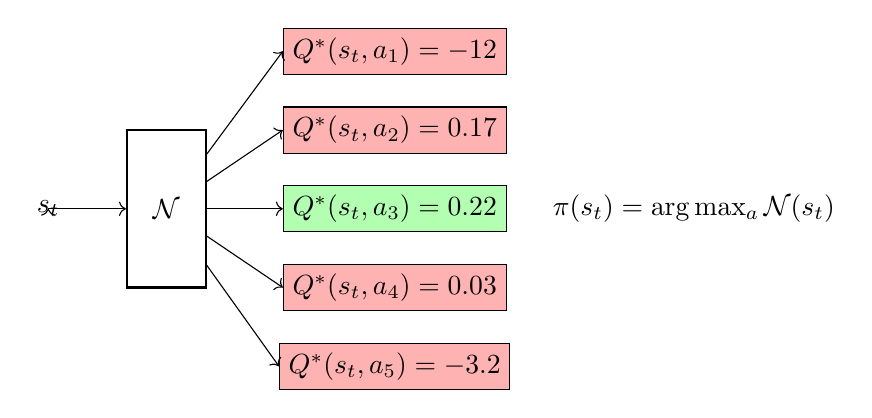
\begin{tikzpicture}
\node[rectangle] at (0,0) {$s_t$};
\node[rectangle] at (1.5,0) [draw,thick,minimum width=1cm,minimum height=2cm] (B) {$\scriptn$};
\node[rectangle] at (4.4, 2)  [draw, fill=red!30] (C1) {$Q^*(s_t,a_1) = -12$};
\node[rectangle] at (4.4, 1)  [draw, fill=red!30] (C2) {$Q^*(s_t,a_2) = 0.17$};
\node[rectangle] at (4.4, 0)  [draw, fill=green!30] (C3) {$Q^*(s_t,a_3) = 0.22$};
\node[rectangle] at (4.4, -1) [draw, fill=red!30]  (C4) {$Q^*(s_t,a_4) = 0.03$};
\node[rectangle] at (4.4, -2) [draw, fill=red!30]  (C5) {$Q^*(s_t,a_5) = -3.2$};
\node[rectangle] at (8.2, 0) (D) {$ \pi(s_t) =  \arg \max_a \scriptn(s_t)$};
\draw[->] (0,0) edge (B);
\draw[->] (B) edge (C1.west);
\draw[->] (B) edge (C2.west);
\draw[->] (B) edge (C3.west);
\draw[->] (B) edge (C4.west);
\draw[->] (B) edge (C5.west);
\end{tikzpicture} 
\end{center}
\end{frame}


%!TEX root = ../pres.tex


\begin{frame}
	\frametitle{Policy Iteration}
	
	\onslide<1->{\textbf{Policy Iteration:} Given access to the MDP, use policy evaluation to iteratively serach for better policies!}
	\begin{itemize}
		\item<1-> Choose a policy at random, $\pi
		$.
		\item<2-> Alternate between
		\begin{itemize}
			\item<2-> Evaluate policy $\pi \to V^\pi$.
			\item<3-> Set new policy to be greedy policy for $V^\pi$
			\begin{equation*}
			\begin{aligned}
				\pi(s) & := \argmax_a \mathbb{E}\left[R(s,a) + \gamma V^{\pi}(s')\right] \\
						& := \argmax_a Q^{\pi}(s, a)
			\end{aligned}
			\end{equation*}
		\end{itemize}
	\end{itemize}
	\onslide<4->{ \emph{Note: Learn $Q^{\pi}$ using Q-learning without $\argmax.$} 
				\begin{equation*}
					Q^{\pi}(s_t,a_t) = r(s_t, a_t) + \gamma Q^{\pi}(s_{t+1}, \pi(s_{t+1})
				\end{equation*}}

\end{frame}


\begin{frame}
  \frametitle{Policy Iteration}
  \textbf{Example: Deep Determisitic Policy Gradient}
  \begin{enumerate}
    \item Actor neural network $\pi_\theta: \scripts \to \scripta$
    \item Critic network $Q^\pi: \scripts \times \scripta \to \mathbb{R}$
    \item Performance of $\pi$ is $Q^\pi(s_t, \pi(s_t))$. \textbf{Maximize performance!} $\nabla_\theta Q^{\pi}(s_t, a_t) = \nabla_a Q^\pi(s_t,a) \cdot \nabla_\theta \pi_\theta(s_t)$
  \end{enumerate}
	\begin{center}
	  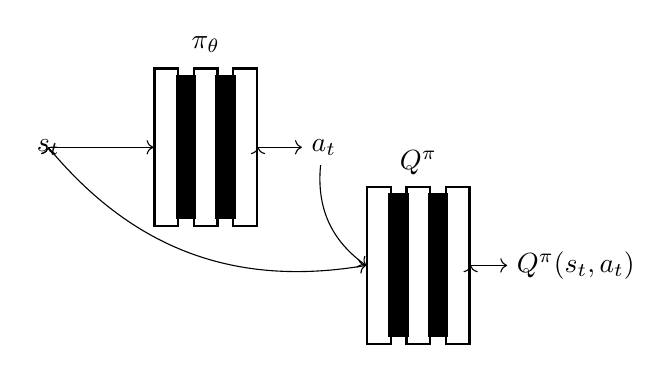
\begin{tikzpicture}
	\node[rectangle] at (0,0)  {$s_t$};
	\node[rectangle] at (1.75,0) [draw,thick,minimum width=0.2cm,minimum height=1.8cm, fill=black] (BC1) {};
	\node[rectangle] at (2.25,0) [draw,thick,minimum width=0.2cm,minimum height=1.8cm, fill=black] (BC2) {};
	\node[rectangle] at (1.5,0) [draw,thick,minimum width=0.3cm,minimum height=2cm] (B1) {};
	\node[rectangle] at (2,0) [draw,thick,minimum width=0.3cm,minimum height=2cm] (B2) {};
	\node[rectangle] at (2.5,0) [draw,thick,minimum width=0.3cm,minimum height=2cm] (B3) {};
	\node[rectangle] at (3.5,0) (action) {$a_t$};
	\draw[->] (B3.east) edge (action.west);
	\node[rectangle] at  (2,1.3) {$\pi_\theta$};
	\draw[->] (0,0) edge (B1);

	\node[rectangle] at (2.7+ 1.75,-1.5) [draw,thick,minimum width=0.2cm,minimum height=1.8cm, fill=black] (QC1) {};
	\node[rectangle] at (2.7+ 2.25,-1.5) [draw,thick,minimum width=0.2cm,minimum height=1.8cm, fill=black] (QC2) {};
	\node[rectangle] at (2.7+ 1.5,-1.5) [draw,thick,minimum width=0.3cm,minimum height=2cm] (Q1) {};
	\node[rectangle] at (2.7+ 2,-1.5) [draw,thick,minimum width=0.3cm,minimum height=2cm] (Q2) {};
	\node[rectangle] at (2.7+ 2.5,-1.5) [draw,thick,minimum width=0.3cm,minimum height=2cm] (Q3) {};
	\node[rectangle] at (2.7+ 2,-1.5 + 1.3) {$Q^\pi$};
	\draw[->, bend right] (0,0) edge (Q1.west);
	\draw[->, bend right] (action) edge (Q1.west);
	\node[rectangle] at (2.7+ 4,-1.5) (critic) {$Q^{\pi}(s_t, a_t)$};
	\draw[->] (Q3.east) edge (critic.west);
	\end{tikzpicture} 
	\end{center}
\end{frame}


\begin{frame}
	\frametitle{$\ $}
	\begin{center}
	\textbf{and many more...}\\
		Papers and links to descriptions of other algorithms will be posted on github.com/mlberkeley/bootcamp.
	\end{center}
\end{frame}

\section{Practice}
%!TEX root = ../pres.tex

\begin{frame}
	\center\huge{Practical Reinforcement Learning}
\end{frame}

\begin{frame}
\frametitle{Process}
\begin{enumerate}
	\item Clearly define the environment.
	\begin{itemize}
		\item What is state space, $\scripts$? Action space $\scripta?$ Low dimensions is better!
		\item Use tools like OpenAI Gym to make a simulator.
	\end{itemize}
	\item Choose a good reward function.
	\begin{itemize}
		\item Don't make sparse reward functions: \\
		\begin{center}
			\textbf{+1 for winning vs. guiding agent to win.}
		\end{center}
		\item Penalize for time constraints!
		\item Break the problem in to smaller goals with rewards $r_1, r_2,\dots$. Then
			$r(s,a) = \sum_i w_i r_i(s,a)$.
	\end{itemize}
\end{enumerate}
\end{frame}


\begin{frame}
\frametitle{Process}
\begin{enumerate}

	\setcounter{enumi}{2}
	\item Choose a model.
	\begin{itemize}
		\item Deep reinforcement learning is king! 
		\begin{itemize}
			\item Discrete $\scripta \to DQN, DDQN$
			\item Continuous $\scripta \to DDPG, NAF, A3C, TRPO.$	
		\end{itemize}
		\item Less hyperparameters better.
		\item Don't rule models out too early.
	\end{itemize}
	\item Train the model against the environment.
	\begin{itemize}
		\item Choose a good exploration strategy.
		\item RL can take a long time (days - months), let models train to completion.
		\item Do a sweep on hyperparameters.
		\item Overfitting (to optimal policy) is good. 
		\item \emph{(You will fail here many times, go to step 3.)}
	\end{itemize}
	\item Profit
\end{enumerate}
\end{frame}



\begin{frame}
\frametitle{$\text{ProTips}^{tm}$}
\begin{itemize}
	\item \textbf{Fastest way to learn RL:} Implement landmark papers in tensorflow, Atari DQN, DPG, ...
	\item \textbf{Write unit tests before you train!}
	\item \textbf{Use an autodiff framework: } Tensorflow, PyTorch, ...
	\item \textbf{Avoid pixel data at all costs: } CNNs/CV algorithms make training very slow!
	\begin{itemize}
		\item Test RL models on featurized data in simualtion, then move to pixel based models for real data.
	\end{itemize}
\end{itemize}
\begin{center}
	\textbf{Good luck!}
\end{center}
\end{frame}


\section{Questions}
\begin{frame}
\Huge{\centerline{Questions?}}
\end{frame}

%----------------------------------------------------------------------------------------

\end{document}
